% !TeX program = xelatex
% COLING 2025-style Chinese draft converted from the confirmed Word manuscript.
% For an actual COLING submission, replace the bundled fallback coling.sty
% with the official coling.sty from the COLING 2025 template archive.
\documentclass[11pt]{article}
\usepackage[review]{coling}
\usepackage{times}
\usepackage{latexsym}
\usepackage{fontspec}
\usepackage{xeCJK}
% Chinese fonts: prefer Noto when available; fall back to Fandol from TeX Live.
\IfFontExistsTF{Noto Serif CJK SC}{%
  \setCJKmainfont{Noto Serif CJK SC}%
}{%
  \setCJKmainfont{FandolSong-Regular}%
}
\IfFontExistsTF{Noto Sans CJK SC}{%
  \setCJKsansfont{Noto Sans CJK SC}%
}{%
  \setCJKsansfont{FandolHei-Regular}%
}
\XeTeXlinebreaklocale "zh"
\XeTeXlinebreakskip = 0pt plus 1pt
\usepackage{microtype}
\usepackage{graphicx}
\usepackage{booktabs}
\usepackage{tabularx}
\usepackage{array}
\usepackage{amsmath,amssymb}
\usepackage{enumitem}
\usepackage{url}
\usepackage{xurl}
\usepackage{multirow}
\usepackage{makecell}
\usepackage{adjustbox}
\setlist{nosep,leftmargin=*}
\title{学习何时思考：面向大语言模型高效推理的自适应反思策略学习}
\author{匿名作者}
\begin{document}
\maketitle
\begin{abstract}
固定反思可以修正部分数学推理错误，但会对已经正确的问题产生不必要的生成成本，也可能引入新错误。本文将反思调用建模为测试时计算分配问题：基础模型先生成初始答案，冻结的小型编码器将问题与初始答案映射为多层隐藏表示，随后由分层策略选择器决定是否调用反思器以及执行一轮还是两轮反思。策略仅使用部署时可获得的文本表示，不依赖人工难度标签、标准答案或候选真实得分；训练监督由离线候选的正确性和输入输出 token 成本构造。

在包含执行失败成本的 GSM8K 1319 题评估中，12 组锁定配置的三种子平均准确率为 94.57--95.30\%，高于 Direct 的 93.33\%；平均总 token 为 406.67--738.46，低于固定一轮反思的 969.72。匹配调用数的随机对照支持策略学习部分反思价值较高的问题，但策略仍低于固定反思和强模型独立回答。跨数据集结果显示，策略在 GSM1K 上有有限迁移，在 SVAMP 上未稳定复现，在 MultiArith 上主要体现为低调用率下维持饱和准确率。本文保留失败成本并报告修复、错误引入和迁移边界；跨数据集结果属于探索性证据。
\end{abstract}
\noindent\textbf{关键词：} 数学推理；大语言模型；自适应反思；策略选择；测试时计算

\section{引言}
大语言模型在简单数学任务上的直接回答准确率已经较高，额外计算的价值因问题而异。当初始回答正确时，再次生成可能只增加开销；当初始回答错误时，反思也可能重复错误。因此，本文的问题不是如何迫使模型频繁反思，而是：\textbf{在存在可修复错误的条件下，能否从问题与初始回答中识别值得反思的问题，并选择合适的反思轮数？}

这一目标要求区分候选能力与选择能力。反思器能否生成更好的答案决定了可利用空间；策略能否在不读取标准答案的情况下选中这些答案决定了实际收益。若完整作答条件下 Direct 已接近上界，则策略选择 Direct 是合理行为，而不是需要通过削弱提示词来纠正的现象。

本文保持 Base、Reflector 和策略选择器解耦的架构。Base 先生成初始回答，Gate 决定是否反思，Round 在反思前决定执行一轮或两轮。基础模型、反思器和小编码器均不更新权重，仅训练轻量分类头。本文的主要工作如下：
\begin{enumerate}
\item 构建数学任务的离线候选监督与在线按需反思流程，明确动作、输入、监督和部署边界。
\item 使用冻结小模型的末层隐藏表示替代人工设计状态特征，并详细说明分层决策、池化方式和可训练参数范围。
\item 审计 thinking、输出预算和评分版本对历史反思收益的影响，统一输入、输出及重试成本。
\item 以有限候选 Oracle、修复/引错分析、配对统计和模型替换对照建立后续验证协议。未完成实验不计入有效性结论。
\end{enumerate}

\section{相关工作}
链式思维通过中间推导支持语言模型推理\cite{wei2022cot}，Self-Consistency 对多个采样路径进行聚合\cite{wang2023selfconsistency}，Tree of Thoughts 将中间状态组织为搜索\cite{yao2023tot}。与固定增加路径数量不同，本文研究样本级计算分配。

Self-Refine 采用反馈和修订循环\cite{madaan2023selfrefine}，Reflexion 使用语言反馈支持后续决策\cite{shinn2023reflexion}。这些机制不意味着任意模型和模板上的反思都有效；完整但错误的解答修正、不完整输出恢复和独立重新作答应分别比较。

GSM8K 的验证器工作强调候选解评价\cite{cobbe2021gsm8k}。本文选择器在部署时不读取候选真实正确性，而从初始文本预测动作。现有算法属于\textbf{离线候选反馈驱动的监督学习}，不是无监督学习或已实现的在线强化学习。奖励用于标签或模型选择，并不会自动使训练成为强化学习。

\section{方法}
\subsection{任务与候选路径}
给定问题 $q$，冻结的基础模型 $M_B$ 生成初始响应
\begin{equation}
y_0=M_B(P_D(q)).
\end{equation}
响应包含模型输出文本；最终数值由答案抽取器单独提取。状态为 $s_0=(q,y_0)$，动作集合为 $\mathcal A=\{D,R_1,R_2\}$。Direct 返回 $y_0$；一轮和两轮路径满足
\begin{equation}
y_1=M_R(P_R(q,y_0,1)),\quad y_2=M_R(P_R(q,y_1,2)).
\end{equation}
同一冻结反思器在一条路径内重复使用。两轮动作返回第二轮答案，不在测试时利用标准答案回选第一轮。不同实验可以替换 $M_R$，但同一组合的生成配置应固定。

图~\ref{fig:framework} 展示完整流程。图中离线候选全部生成，线上只执行选中的路径。当前新对照为两种反思器采用相同的响应条件模板，第一轮读取初始回答，第二轮读取第一轮可见回答。历史模板有一版明确隐藏原回答，属于独立重新作答，不能与该机制混称。
\begin{figure*}[t]
\centering
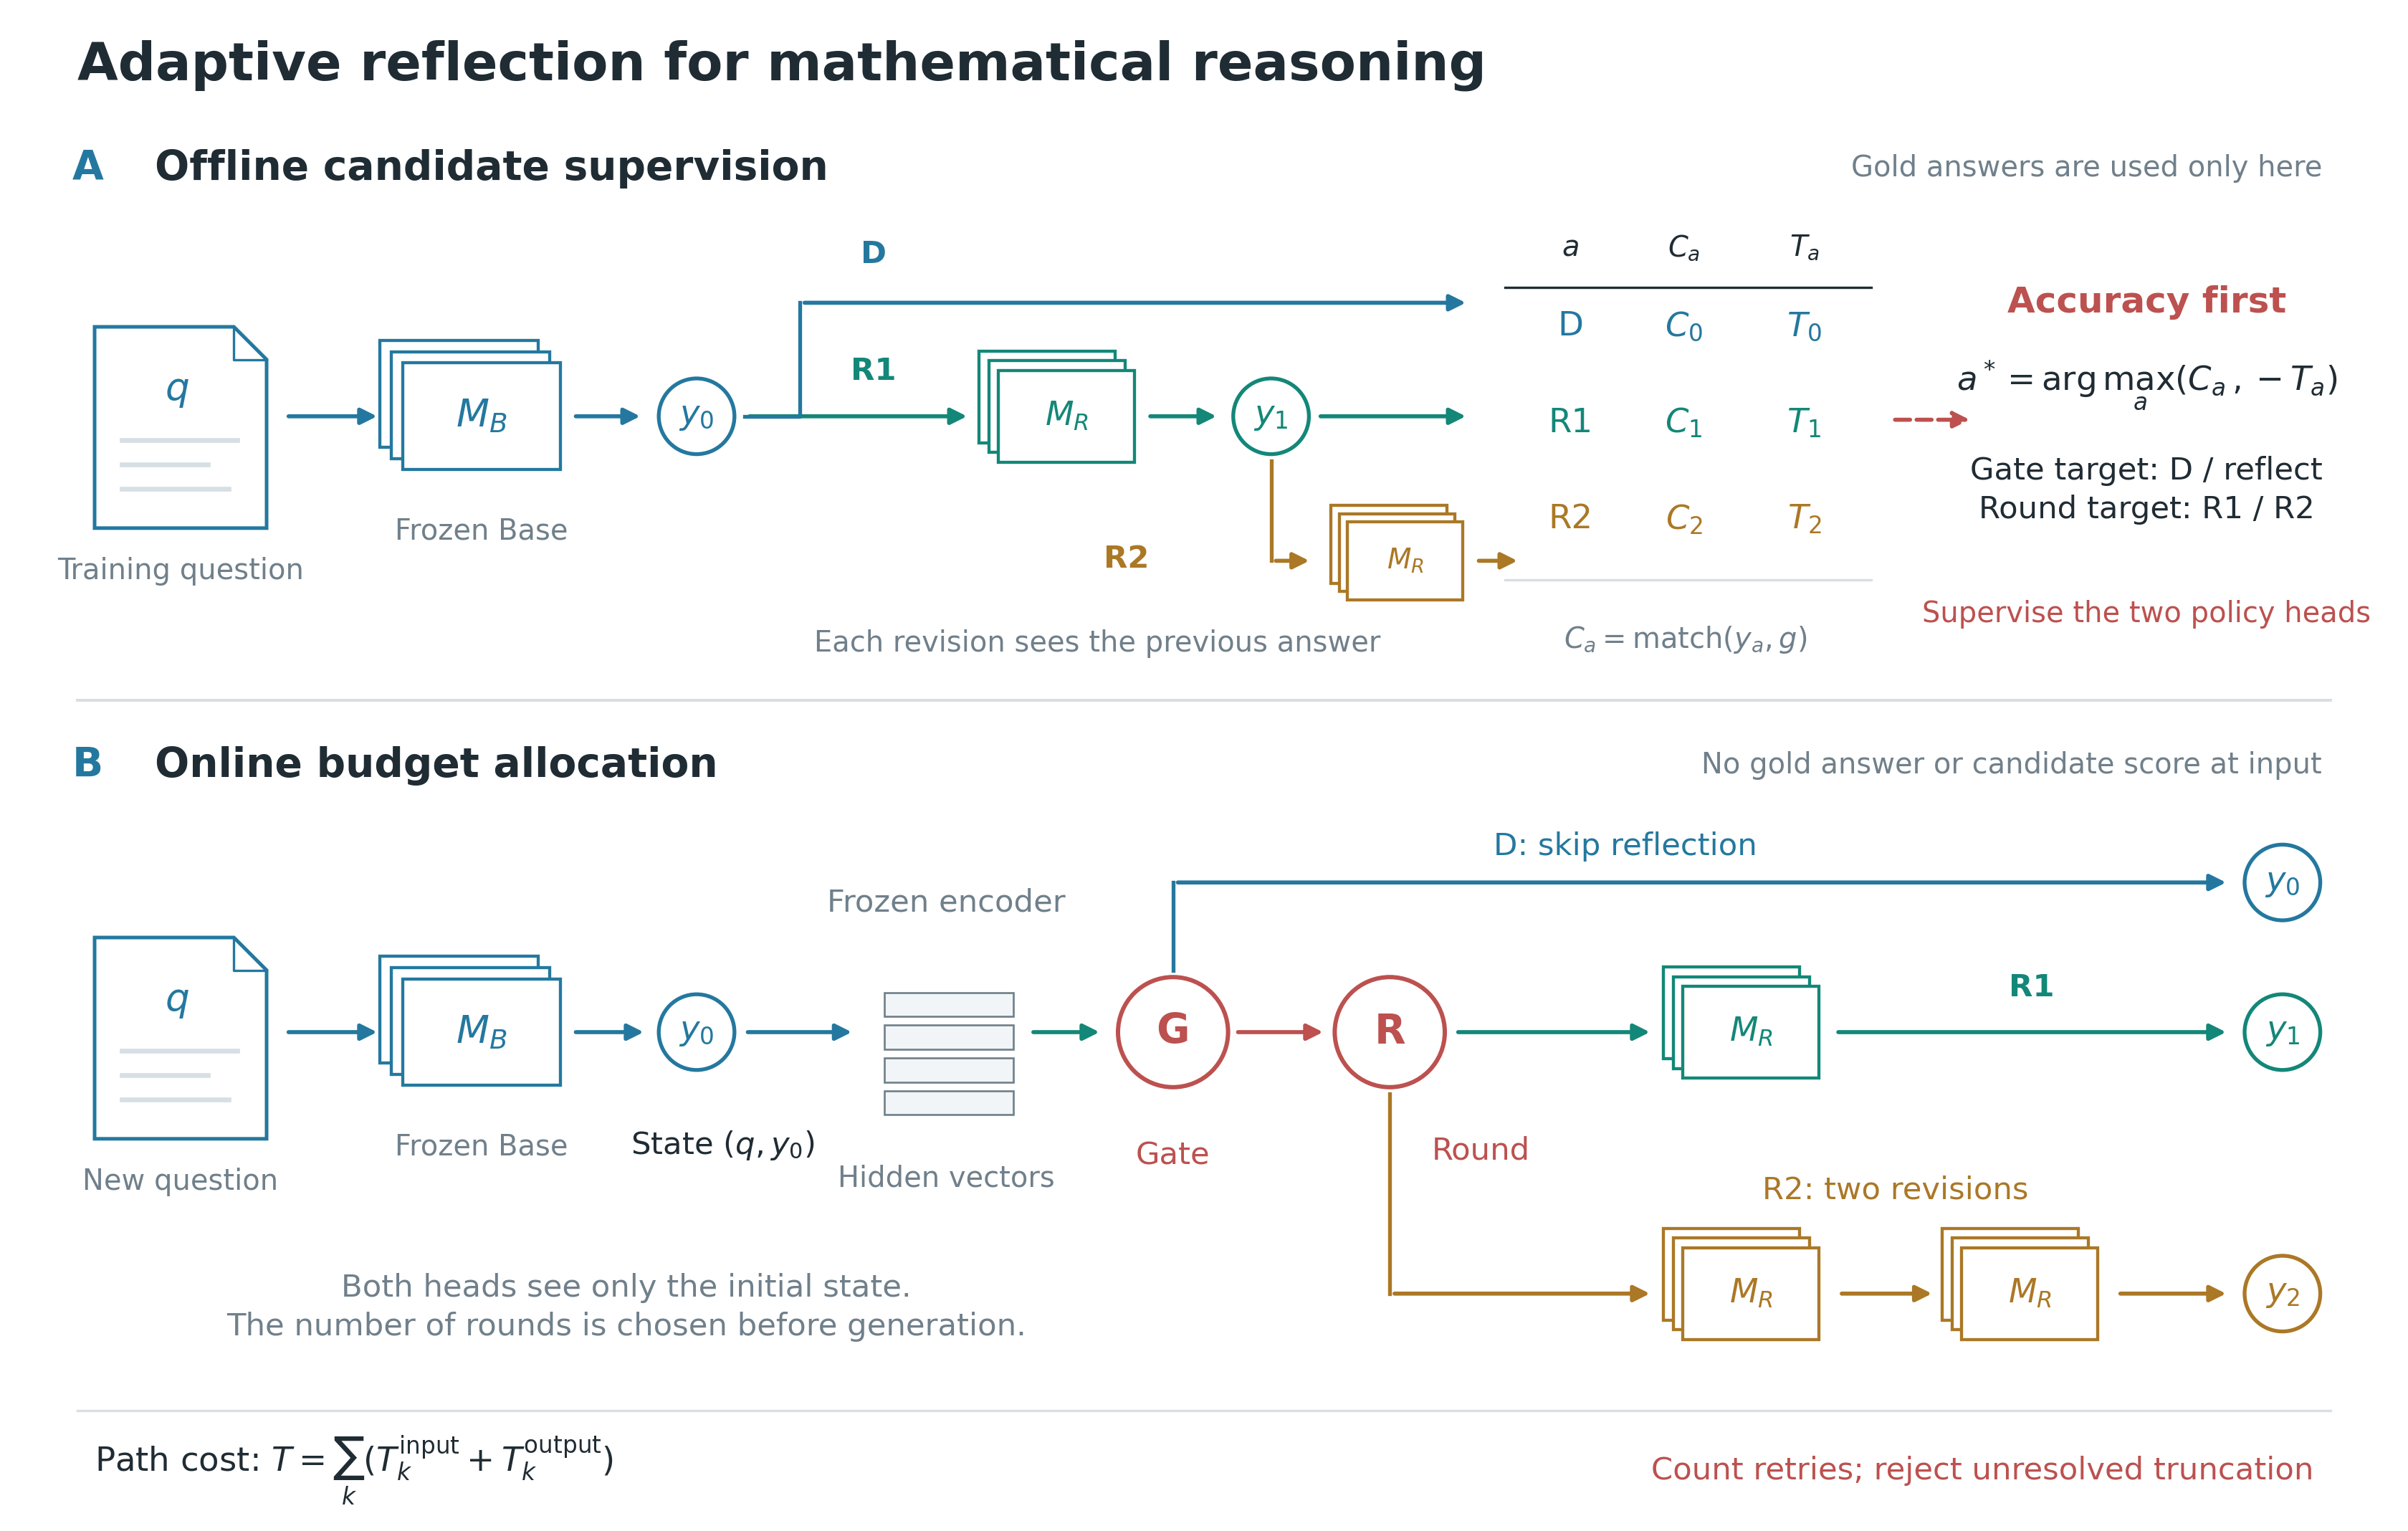
\includegraphics[width=\textwidth]{figures/adaptive_reflection_framework.png}
\caption{数学自适应反思框架。上半部为离线候选评分和监督目标；标准答案 $g$ 仅用于正确性判定。下半部为部署路径：两个策略头均根据初始状态决策，Direct 绕过反思器，R1/R2 分别执行一次/两次修订。$M_B$ 与 $M_R$ 均冻结；图中的重复模型符号表示调用，不表示独立训练的副本。}
\label{fig:framework}
\end{figure*}

\subsection{离线监督与准确率优先目标}
对候选 $a$ 保存最终响应、抽取答案、正确性 $C_a\in\{0,1\}$ 与累计成本 $T_a$。主模型采用字典序目标
\begin{equation}
a^*=\mathop{\arg\max}_{a\in\mathcal A}(C_a,-T_a).
\label{eq:accfirst}
\end{equation}
先比较正确性，再在同正确性候选中选择较低成本。若仍相同，按固定动作顺序打破平局。成本敏感消融使用
\begin{equation}
r_a=C_a-\lambda T_a,\qquad a^*_{\lambda}=\mathop{\arg\max}_a r_a.
\label{eq:reward}
\end{equation}
用于标签的 $\lambda$ 和仅用于汇总报告的 $\lambda$ 应分别记录。即使主模型不使用成本敏感标签，也可以报告其在固定 $\lambda$ 下的平均奖励。

完整训练轨迹可在不重新调用大模型的条件下重标注。direct-first 选择性构造仅对 Direct 错误题生成反思；当 Direct 已正确且额外调用有正成本时，式~\ref{eq:accfirst} 可将其标为 D。但这些问题缺少反思观测，不能将缺失结果当作错误或零成本，不能据此计算固定反思准确率、错误引入率或完整候选 Oracle。新的正式测试比较需要所有待评动作的完整覆盖。

\subsection{Gate 与 Round 的分层决策}
令最优反思动作及门控标签为
\begin{equation}
r^*=\mathop{\arg\max}_{a\in\{R_1,R_2\}}(C_a,-T_a),\quad g^*=\mathbf{1}[a^*\ne D].
\end{equation}
Gate 学习 D 与反思之间的二分类；Round 学习 R1 与 R2 之间的二分类。Round 训练使用具有两种反思候选的题目，不只限于 Gate 正类；对缺少反思候选的题目不伪造轮次标签。两个头独立训练，不存在共享梯度更新的联合训练编码器。

令 $p_D$ 为 Gate softmax 对 D 的输出，$p_{R_1}$、$p_{R_2}$ 为 Round 分数，则基本决策为
\begin{equation}
\pi(s_0)=\begin{cases}
D,&p_D(s_0)\geq\tau_G,\\
\arg\max_{a\in\{R_1,R_2\}}p_a(s_0),&\text{otherwise}.
\end{cases}
\label{eq:policy}
\end{equation}
门限在训练侧验证部分确定。分数不是已证明校准的正确概率；门控标签表示相对候选优势，也不等于初始答案是否错误。

这种分层方式将“要不要额外计算”与“分配多少额外计算”分开，便于解释和消融，但不保证优于平坦三分类。尤其是 Round 在看到第一轮新结果前就决定预算，本文不是逐轮更新状态的序贯控制或强化学习。

\subsection{冻结编码器与高维向量}
按照固定文本模板连接 Question 与 Initial answer，得到 token 序列 $t_{1:L}$ 及有效位置掩码 $m_i$。纯文本策略不输入人工难度、置信度、verifier 得分、标准答案、正确性或奖励。训练监督标签与输入特征是两回事。

编码器为 Qwen3-0.6B-Base，共 28 个 Transformer block，隐藏宽度 $d=1024$。\textbf{词嵌入、全部 block 和最终归一化均不训练}。实现以 eval 模式和 no-grad 前向提取隐藏状态，只有后续 MLP 出现在优化器中。最后两层被读取，不是被解冻；亦不使用语言模型词表输出头来生成动作文本。

令 $H^{(\ell)}\in\mathbb R^{L\times d}$ 为读取的隐藏状态，$i^*$ 为最后一个有效 token 位置。每层计算
\begin{equation}
\mu^{(\ell)}=\frac{\sum_i m_iH_i^{(\ell)}}{\sum_i m_i},\quad v^{(\ell)}=H_{i^*}^{(\ell)}.
\end{equation}
取 $S=\{-2,-1\}$，按实现顺序拼接
\begin{equation}
z=[\mu^{(-2)};v^{(-2)};\mu^{(-1)};v^{(-1)}]\in\mathbb R^{4096}.
\label{eq:vector}
\end{equation}
mean 聚合有效位置的表示，last 读取最后位置的上下文化状态；二者是建模选择，而不是保证可辨识错误的理论充分统计量。向量维度由层数、隐藏宽度和池化决定，与样本数不存在相等关系。最后三层采用同样方式会得到 6144 维，但不意味着微调三个 block。

当前策略编码上限为 1024 token，并启用 tokenizer 截断；它与生成模型的 32768 上下文及输出预算不同。完整生成响应仍可能在策略输入中被截短。正式实验应记录策略输入截断比例，检查是否丢失最终答案，并仅在开发数据上决定长度配置，不能把“生成无未解决截断”写成“整个系统没有截断”。

\subsection{分类头与学习过程}
两个头分别使用仅在各自训练部分拟合的 StandardScaler。标准化后输入 $4096\rightarrow64\rightarrow16\rightarrow2$ 的 MLP，两层隐藏层使用 ReLU，输出为两个 logits，经 softmax 得到动作分数。每个头包含 263,282 个可训练参数，合计 526,564 个；不含冻结编码器参数和非梯度的 scaler 统计量。

对头 $h\in\{G,R\}$，使用交叉熵
\begin{equation}
\mathcal L_h=-\sum_{i\in\mathcal D_h}w_{h,y_i}\log p_h(y_i\mid z_i).
\end{equation}
历史主脚本中 Gate 不启用类别权重，Round 使用训练类别频数计算权重。训练以 AdamW 更新各自 MLP；编码器没有梯度回传。图~\ref{fig:network} 中红色只表示可训练分类头，蓝绿张量色块是结构示意，不是实际激活值或特征重要性热图。
\begin{figure*}[t]
\centering
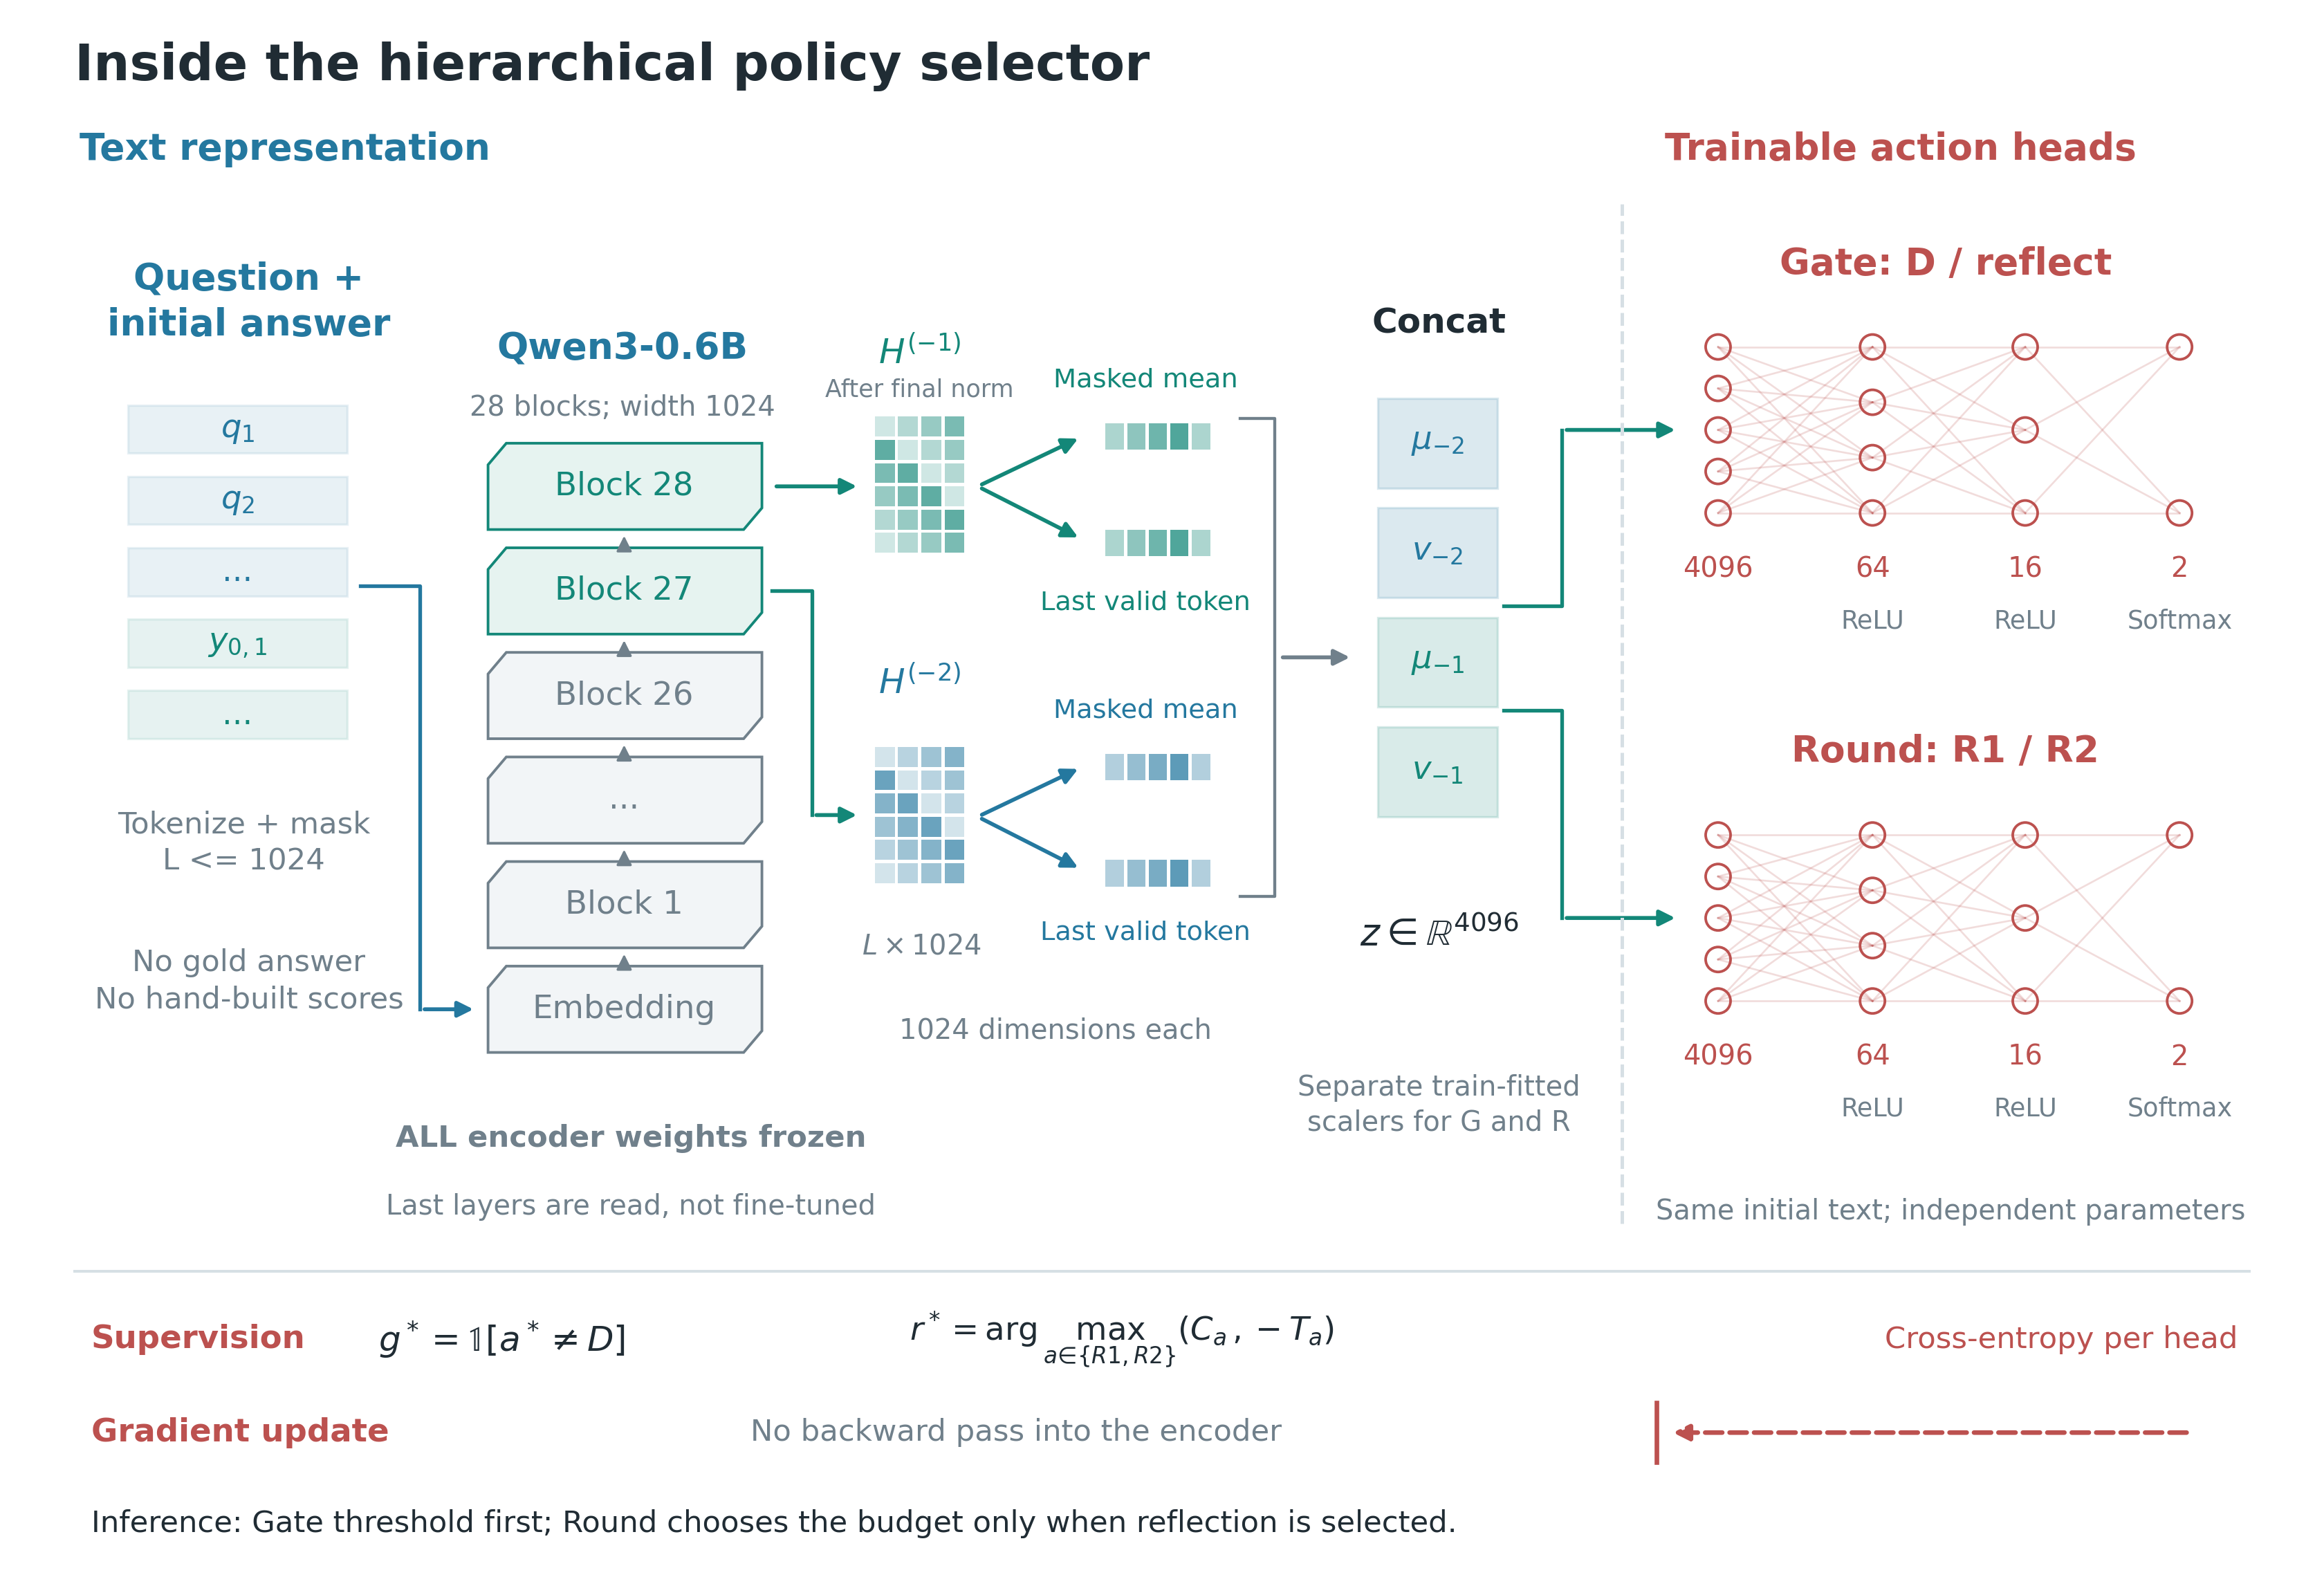
\includegraphics[width=\textwidth]{figures/adaptive_reflection_policy_network.png}
\caption{数学策略选择器网络。输入文本先经过完全冻结的 28 层编码器，读取最后两层，分别做 masked mean 和 last-valid-token 池化，拼成 4096 维向量。两个独立 scaler 与 MLP 分别学习 Gate 和 Round。虚线边界区分冻结表示与可训练头；底部红色箭头只表示头部反向更新，不进入编码器。神经元数目经过示意压缩，真实维度以数字标注。}
\label{fig:network}
\end{figure*}

动作准确率与最终答案准确率不相同：多个动作都可能答对，偏离最优动作也可能产生正确答案。全选 D 的分类器还可能因类别不平衡取得较高标签准确率，因此同时记录动作指标、最终回答准确率、成本及错误转移。

\subsection{路径成本与完整性}
对实际执行调用集合 $\mathcal C(q)$ 定义
\begin{equation}
T(q)=\sum_{k\in\mathcal C(q)}(T_k^{\mathrm{in}}+T_k^{\mathrm{out}}).
\label{eq:cost}
\end{equation}
R1 包含 Base 和第一轮，R2 再加第二轮；每条独立路径中的 Base 只计一次。重复送入反思器的文本属于新输入。输出触限后重试产生的所有可计量输入、输出也须累计，不能只记录最后一次成功调用。

主策略不包含 verify-reflect 动作，也没有在线 LLM verifier。标准答案评分是离线监督或测试过程，不是部署调用。小编码器虽不产生生成式 token，仍有前向计算开销，应另报延迟、显存和吞吐。跨模型 token 不等价于同量 FLOPs 或相同费用。

有限预算不能保证模型绝不触限。当前对照采用严格失败保护：记录每次调用的 finish reason 与 usage；length 结束按预定预算重试；达到最大预算仍不完整则停止并保留轨迹，不将其写为普通语义错误或悄悄丢弃。最终评测须报告无法解决的失败数。格式检查不读取标准答案，自然停止也不等于答案正确。

\section{实验协议}
\subsection{数据与研究边界}
GSM8K 训练集 7473 题、测试集 1319 题为数学主任务。历史迁移评测使用项目处理后的 GSM1K 1205 题、SVAMP 300 题和 MultiArith 180 题，这些数字不是对各原始数据集完整规模的声明。后续迁移保持策略与生成协议锁定，难度桶作为报告分组，不作为纯文本策略输入。

新反思器开发对照使用训练侧固定 200 题，按 seed=20260910 的 ID 哈希排序抽取，选择过程不读取正确性或奖励，并排除与官方测试的 ID/规范化问题重叠。该训练池历史上已使用，因此是探索性开发集，不是独立确认测试。

\subsection{模型与对照}
基础模型使用本地别名 Qwen3-8B-Instruct；旧反思器为 DeepSeek-R1-Distill-Qwen-7B，新候选为 Qwen/Qwen3-14B。后者已从 ModelScope 下载并校验，但完成下载并不证明反思更强。当前开发协议中 Base 显式关闭 thinking，DeepSeek 保留原生模板，Qwen3-14B 启用 thinking，因此比较的是完整模型配置，而不是单独参数规模的因果效应。

两个反思器共享相同 Base 响应和响应条件提示。另设 Qwen3-14B 独立重新作答，不向其提供 Base 回答；分别报告独立调用成本以及 Base 后再独立作答的总成本，以辨别反思是否优于普通的额外生成。历史全冻结策略不会因为更换反思器而自动变成已验证的新策略，正式主实验仍需重新检查标签和分布一致性。

各角色使用 32768-token 上下文，输出预算依次为 4096、8192、16384；每次请求前要求
\begin{equation}
L_{\mathrm{input}}+16384+512\leq32768.
\end{equation}
这里的输入长度按实际角色 tokenizer 与 chat template 计算，反思输入在上一轮响应确定后再检查。输入过长时停止，不通过静默裁剪来通过检查。提示文本与哈希、模型元信息、解码设置、评分实现和代码指纹均保存；模型 revision 的完整发布信息仍需在投稿前整理。

\subsection{训练、epoch 与验证}
历史数学策略采用 80/20 训练/验证，种子为 7、21、42，AdamW 学习率和 weight decay 均为 $10^{-3}$，头部 batch size 为 128，训练 10 个 epoch。Gate/Round 的编码 batch size 分别为 8/4，输入上限 1024，隐藏层为 64、16。

历史脚本以验证答案准确率选择 epoch，同值保留最早轮，再进行验证门限校准。Gate 的验证答案指标用最优反思候选作为反思代表，是乐观子任务指标，不等于实际 Round 组合后的系统准确率。历史两个头按不同标签各自分层划分，因此后续正式确认须使用\textbf{共享的问题级训练/验证清单}，组合校准不能读取任何一个头已经训练过的问题。当前图展示网络结构，不声称这一协议改进已完成。

\begin{table}[t]
\centering\small
\caption{历史主配置的 epoch 记录；选择依据来自训练历史而非测试得分。}
\label{tab:epochs}
\begin{tabular}{rrrr}
\toprule
Seed & 总 epoch & Gate & Round\\
\midrule
7 & 10 & 1 & 1\\
21 & 10 & 1 & 5\\
42 & 10 & 1 & 2\\
\bottomrule
\end{tabular}
\end{table}

\subsection{评价与统计}
数学评价以任务适用的数值或等价判断计算准确率，不采用词级 F1。报告平均输入 token、输出 token、总成本、反思调用率与固定 $\lambda$ 下的奖励。有限候选 Oracle 按式~\ref{eq:accfirst} 回溯选择，仅是既定候选池的上界，不能部署，也不代表更换模型、提示或增加采样后的理论上限。

同题比较使用配对 Bootstrap，按问题重采样 10,000 次，报告差值的 95\% 区间；二值正确性另用双侧精确 McNemar 检验。三策略种子的标准差描述训练随机性，不等于独立重采样 LLM 轨迹；同题多种子输出不能视作相互独立的新问题。未显著不代表等效，若要求保证准确率，应事先定义非劣容许差。

历史测试集已反复被查看，多种子和统计检验不能消除这种开发反馈。新权重、门限、提示和候选配置只在训练侧开发部分选择，在正式测试前锁定；测试 Oracle 仅用于解释差距，不用于反复调参。

\section{已有结果与生成审计}
\subsection{历史候选上的策略选择}
\begin{table}[t]
\centering\small
\caption{历史 GSM8K 1319 题轨迹，存在 thinking/输出预算混杂，不作为新完整输出主实验。误差为三个策略种子的标准差。}
\label{tab:historical}
\resizebox{\columnwidth}{!}{%
\begin{tabular}{lccc}
\toprule
方法 & 准确率 & 平均 Token & 反思率\\
\midrule
Direct & 0.5588 & 547.4 & 0.0000\\
Fixed R1 & 0.8810 & 1683.2 & 1.0000\\
Fixed R2 & 0.8916 & 2683.2 & 1.0000\\
准确率优先分层策略 & $0.8926\pm0.0062$ & $1475.4\pm196.7$ & 0.5365\\
成本敏感分层策略 & $0.8848\pm0.0013$ & $1235.2\pm13.8$ & 0.5363\\
有限候选 Oracle & 0.9212 & 1033.0 & 0.3624\\
\bottomrule
\end{tabular}}
\end{table}

表~\ref{tab:historical} 中准确率优先策略相对 Fixed R2 少用约 45.0\% token；成本敏感版本的标签 $\lambda=5\times10^{-5}$，相对 Fixed R1 少用约 26.6\%。这些结果说明在历史固定候选内可以学习更低成本的选择，不能解释成同等完整作答条件下的巨大推理提升。

\subsection{Base 预算与模型规模混杂}
旧 1319 题审计中，8B Direct 准确率 0.5588，4B 为 0.9189；题目、标准答案及字面 Direct 提示已对齐，但 thinking 行为和 checkpoint 发布代际不等价。8B 输出触及 512 token 的比例为 0.5375，4B 为 0.0167。旧轨迹未完整保存 finish reason，因此这是触限代理，不是对所有截断的直接观测。

8B 未触限的 610 题上，8B/4B 准确率为 0.9918/0.9803；触限的 709 题上为 0.1862/0.8660。4B 正确但 8B 错误的 493 题全部位于 8B 触限组，其中 486 题缺少最终答案标记。8B 的 582 个 Direct 错误中，一轮反思修复 432 个，全部来自触限组。该诊断不足以证明每题的因果机制，但足以否定将旧差距直接归因于参数规模的解释。

统一非 thinking 配置并对 100 题一致重评分后，8B/4B Direct 准确率为 0.93/0.95，没有触限样本。8B 原存分为 0.87，其中 6 题因评分一致化变为正确。这个小规模诊断不是完整主结果，也不证明两个模型等效。

\subsection{重建数据仍需完整性核验}
旧非 thinking 重建的 7473 题中，Direct 正确 6976（0.9335），错误 497。v4 分析仅在这些错误题中记录 R1 修复 241、R2 修复 244、并集修复 309。它们是训练侧数据，不是测试准确率；正确题没有全量反思观测，无法估计错误引入。

进一步核验发现该 Base 文件仍有 26 次 length 结束和 28 个缺少最终答案标记的响应；v4 反思分析有 87 次 length 调用，严格格式通过率为 39.94\%。此外 v4 模板明确不展示此前答案，应称为独立重新作答。新 200 题对照重新生成共享 Base 并使用显式响应条件模板，不能把新旧候选在未审计情况下合并。

\subsection{修复、引错与难度}
对任一方法 $a$，分别定义
\begin{equation}
\mathrm{FixRate}_a=\frac{N(C_0=0,C_a=1)}{N(C_0=0)},\quad
\mathrm{HarmRate}_a=\frac{N(C_0=1,C_a=0)}{N(C_0=1)}.
\end{equation}
两者分母不同，不能直接相减得到总体增益；准确率差为 $(N_{\mathrm{fix}}-N_{\mathrm{harm}})/n$。若分母为零应报告不适用。question-only 难度划分是复杂度代理，阈值在训练侧固定，不是人工难度金标准。

历史 hard 组共 278 题，Direct 错误 183、正确 95；R1 修复/引错为 133/1，R2 为 134/3，同样受预算混杂影响。新的错误分析需区分输出不完整、可恢复格式错误、完整响应的算术或条件理解错误，并在所有问题都有候选时统计引错。

\section{受控实验与预留结果}
\subsection{先检验反思候选空间}
固定 200 题开发对照比较共享 Base 下的两个反思器、独立重新作答以及有限候选 Oracle。首先判断完整作答条件下是否存在足够的净修复空间，再训练策略。若更强模型独立解题已经达到同样效果，不能将额外收益独占归因于反思机制。截止本稿，试验尚未形成完整对照，不能填入有效性数字。

\begin{table*}[t]
\centering\small
\caption{固定 200 题训练侧开发对照预留。未完成不记为零；该表不替代正式测试。}
\label{tab:pilot}
\begin{tabular}{lrrrrr}
\toprule
配置 & Acc. & 输入 Token & 输出 Token & 总 Token & 修复/引错\\
\midrule
共享 Base Direct & -- & -- & -- & -- & --/--\\
DeepSeek R1 & -- & -- & -- & -- & --/--\\
DeepSeek R2 & -- & -- & -- & -- & --/--\\
Qwen3-14B R1 & -- & -- & -- & -- & --/--\\
Qwen3-14B R2 & -- & -- & -- & -- & --/--\\
Qwen3-14B 独立解题 & -- & -- & -- & -- & --/--\\
Base 后接 Qwen3-14B 独立解题 & -- & -- & -- & -- & --/--\\
DeepSeek / Qwen3-14B 有限候选 Oracle & -- & -- & -- & -- & --/--\\
\bottomrule
\end{tabular}
\end{table*}

\subsection{主实验、迁移与消融}
正式主实验以准确率优先分层策略为主模型，对照 Direct、固定 R1/R2、RF 人工特征基线和平坦向量三分类。保持同题候选一致，通过离线回放比较策略；只要协议、完整性及成本可追溯，就无需为每个策略重复调用大模型。

\begin{table}[t]
\centering\small
\caption{完整输出条件下 GSM8K 1319 题主实验预留，尚未完成。}
\label{tab:main-pending}
\resizebox{\columnwidth}{!}{%
\begin{tabular}{lrrrr}
\toprule
方法 & Acc. & 输入/输出 Token & 总 Token & 反思率\\
\midrule
Direct & -- & --/-- & -- & --\\
Fixed R1 & -- & --/-- & -- & --\\
Fixed R2 & -- & --/-- & -- & --\\
RF（人工特征） & -- & --/-- & -- & --\\
向量 MLP（三分类） & -- & --/-- & -- & --\\
Gate--Round（主模型） & -- & --/-- & -- & --\\
有限候选 Oracle & -- & --/-- & -- & --\\
\bottomrule
\end{tabular}}
\end{table}

\begin{table}[t]
\centering\small
\caption{后续数学验证清单。只报告实际完成的项目。}
\label{tab:next}
\resizebox{\columnwidth}{!}{%
\begin{tabular}{lll}
\toprule
项目 & 固定条件 & 待报告\\
\midrule
三个随机种子 & 同一候选及验证清单 & 均值、标准差、配对区间\\
反思器替换 & 共享 Base 响应 & 修复、引错、成本\\
独立重新作答 & 同题、同计费口径 & 机制差异和准确率差\\
数学迁移 & 不在目标测试上调参 & Acc.、反思率、成本\\
表示与结构消融 & 相同训练/验证问题 & 层数、pooling、平坦/分层\\
hard 分组 & 完整正确/错误候选 & 修复率、引错率、错误类型\\
输入与部署审计 & 固定硬件/并发 & 编码截断率、延迟、显存\\
\bottomrule
\end{tabular}}
\end{table}

替换反思器后重新训练策略，验证的是组件可替换性和再适配；同一冻结策略直接用于新反思器，才属于无需再训练的迁移。跨数学数据集迁移采用同样区分。简单数据集若无明显修复空间，应报告高 Direct 基线与低调用率，而不是以降低 Base 作答质量制造改进。

\section{讨论与结论}
本文将数学反思拆分为候选生成和轻量预算选择，在固定大模型的条件下，通过冻结小模型的隐藏表示训练 Gate 和 Round。其价值应体现为完整作答条件下可重复的准确率与计算成本权衡，而不是仅提高动作分类准确率或从测试 Oracle 反推门限。

历史结果显示了条件性的候选选择能力，但审计揭示 thinking、输出预算和评分变化构成重要混杂。当前阶段不能宣称已经完成无混杂的主实验。后续将以锁定的准确率优先策略、完整候选覆盖、模型替换与独立作答对照验证核心假设；如果反思候选本身没有净收益，则不应期待选择器凭空创造收益。

\section{Limitations}
\begin{enumerate}
\item 历史测试被多次查看，后续冻结、三种子与显著性分析不能追溯消除选择偏差。
\item 旧输出预算触限只能提供部分截断证据；新候选比较尚未完整完成，不能把训练侧诊断当测试结果。
\item 选择性训练缺少 Direct 正确题的反思结果，可能低估有害修订风险；正式测试必须完整覆盖。
\item 最后两层表示、mean/last 池化及分层结构属于经验选择，不保证动作可分性、概率校准或语义可解释性。
\item 生成长度保护不等于策略编码无截断；1024-token 编码窗口需要单独审计。
\item token 不覆盖小策略全部计算成本，也不等价于跨模型 FLOPs、费用或端到端加速。
\item ID/文本去重不能排除语义近重复或预训练污染；原生 thinking、tokenizer 和模型代际差异限制因果归因。
\end{enumerate}

\section{Ethics Statement}
本文使用公开数学推理数据，不新增采集用户私有信息。数据排除规则、失败数和评分方式应随结果披露，不能依据测试结果删除困难题。标准答案仅用于离线监督与评估；Oracle 为不可部署参照。反思可能引错，本框架不保证答案正确，不把待完成实验或不显著结果写成已验证成功。

\begin{thebibliography}{99}
\bibitem[Wei et al.(2022)]{wei2022cot} Jason Wei et al. Chain-of-Thought Prompting Elicits Reasoning in Large Language Models. \url{https://arxiv.org/abs/2201.11903}.
\bibitem[Wang et al.(2023)]{wang2023selfconsistency} Xuezhi Wang et al. Self-Consistency Improves Chain of Thought Reasoning in Language Models. ICLR 2023. \url{https://arxiv.org/abs/2203.11171}.
\bibitem[Yao et al.(2023)]{yao2023tot} Shunyu Yao et al. Tree of Thoughts: Deliberate Problem Solving with Large Language Models. NeurIPS 2023. \url{https://arxiv.org/abs/2305.10601}.
\bibitem[Shinn et al.(2023)]{shinn2023reflexion} Noah Shinn et al. Reflexion: Language Agents with Verbal Reinforcement Learning. \url{https://arxiv.org/abs/2303.11366}.
\bibitem[Madaan et al.(2023)]{madaan2023selfrefine} Aman Madaan et al. Self-Refine: Iterative Refinement with Self-Feedback. \url{https://arxiv.org/abs/2303.17651}.
\bibitem[Cobbe et al.(2021)]{cobbe2021gsm8k} Karl Cobbe et al. Training Verifiers to Solve Math Word Problems. \url{https://arxiv.org/abs/2110.14168}.
\end{thebibliography}

\appendix
\section{真实训练曲线与检查点}
图~\ref{fig:curves} 直接来自保存的数学 seed 7 训练曲线，不合成、平滑替换或将示意曲线当真实训练。Gate 训练 loss 从 0.2473 降到 0.0164，验证 loss 从 0.2801 升到 0.8319；Round 验证 loss 从 0.6301 升到 3.2173，呈现明显过拟合迹象。

Gate 的验证答案准确率保持 0.9431，是最优反思代表和门限校准共同作用下的子任务指标，不表示端到端部署准确率。首次最大值规则选择 epoch 1，之后仍需与实际 Round 组合校准。图中的动作准确率、答案准确率与 reward 应按图例分别阅读。
\begin{figure*}[t]
\centering
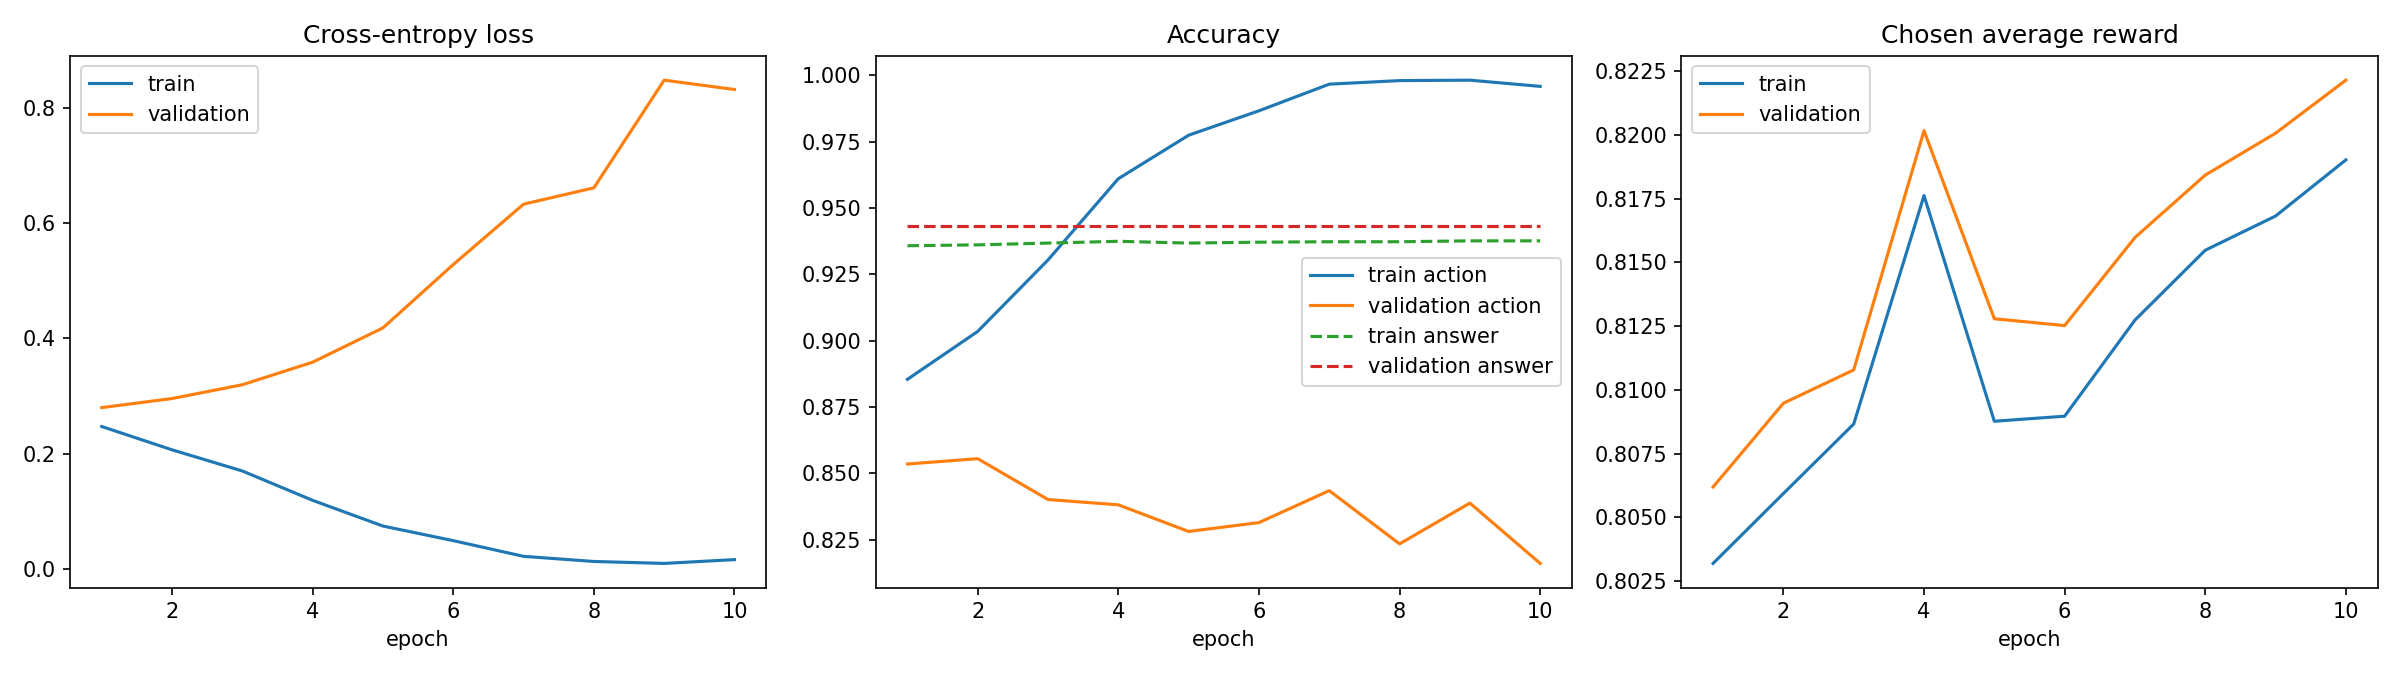
\includegraphics[width=0.95\textwidth]{figures/math_gate_seed7.png}
\par\medskip
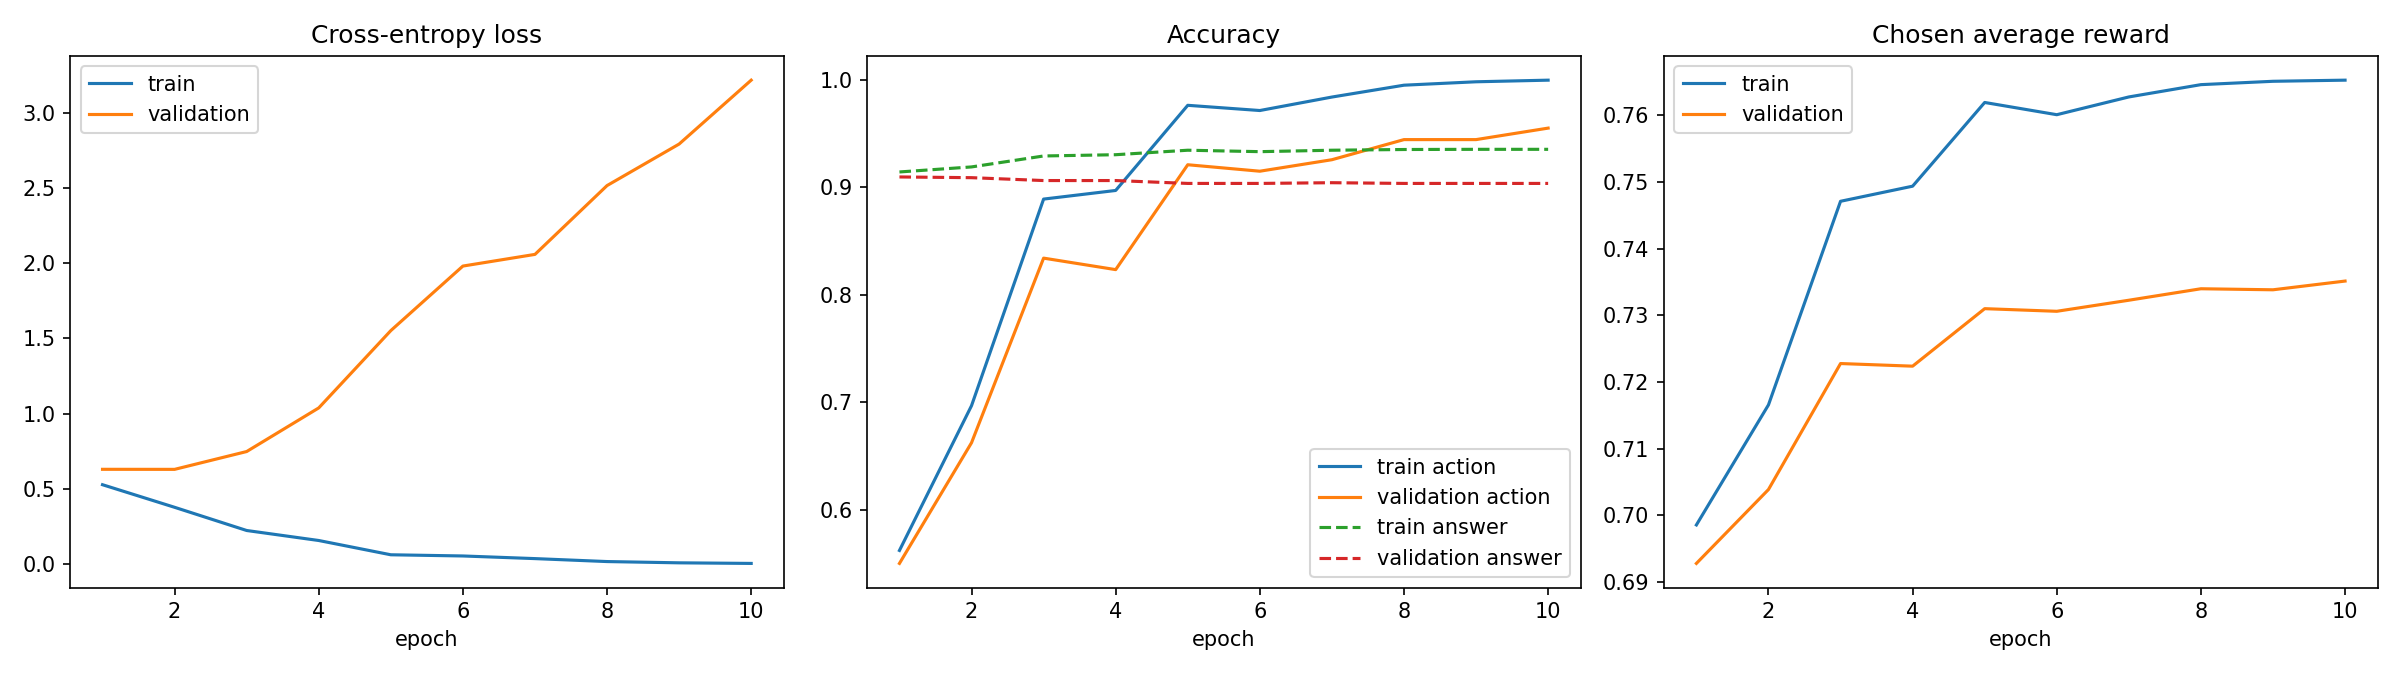
\includegraphics[width=0.95\textwidth]{figures/math_round_seed7.png}
\caption{历史数学 Gate（上）与 Round（下），seed 7。为训练诊断而非新的测试结果；两张图均使用真实保存曲线。}
\label{fig:curves}
\end{figure*}

\section{历史数学迁移}
以下结果仅作为历史成本敏感策略（标签 $\lambda=5\times10^{-5}$）的可追溯记录，尚未统一重做生成审计。它们不替代新的受控迁移，也不意味着研究过程中从未查看目标测试反馈。
\begin{table}[t]
\centering\small
\caption{历史数学迁移；误差为策略种子标准差。}
\label{tab:transfer}
\resizebox{\columnwidth}{!}{%
\begin{tabular}{lrrrr}
\toprule
数据集 & 策略 Acc. & R1 Acc. & 策略 Token & R1 Token\\
\midrule
GSM1K & $0.8595\pm0.0013$ & 0.8548 & $1411.9\pm20.9$ & 1760.0\\
SVAMP & $0.9000\pm0.0033$ & 0.8833 & $908.8\pm23.9$ & 1506.0\\
MultiArith & 0.9833 & 0.9833 & $435.4\pm2.9$ & 1268.9\\
\bottomrule
\end{tabular}}
\end{table}

\begin{table}[t]
\centering\small
\caption{历史成本敏感策略减 Fixed R1 的配对差值及 95\% Bootstrap 区间；未经多重比较校正。}
\label{tab:bootstrap}
\resizebox{\columnwidth}{!}{%
\begin{tabular}{lcc}
\toprule
数据集 & Acc. 差 [CI] & Token 差 [CI]\\
\midrule
GSM8K & $0.0038\ [-0.0010,0.0088]$ & $-448.1\ [-478.2,-417.9]$\\
GSM1K & $0.0047\ [-0.0014,0.0108]$ & $-348.1\ [-380.3,-315.2]$\\
SVAMP & $0.0167\ [0.0044,0.0322]$ & $-597.2\ [-656.0,-537.3]$\\
MultiArith & $0.0000\ [0.0000,0.0000]$ & $-833.5\ [-861.5,-802.5]$\\
\bottomrule
\end{tabular}}
\end{table}
GSM8K/GSM1K 的准确率差区间包含 0，不构成统计等效证明；MultiArith 的退化区间只反映有限样本上观测差为零。SVAMP 正向区间属于探索证据，不能推广到所有数学多步问题。

\section{复现来源与稿件状态}
网络对应 \path{src/transformer_policy.py}、\path{src/neural_policy.py} 与 \path{scripts/run_hierarchical_multiseed.sh}。历史主结果位于 \path{outputs/multiseed/gsm8k_hierarchical_accuracy/summary.json}；训练曲线位于 \path{outputs/training_curves/multiseed/}。

预算审计见 \path{outputs/decoupling_full_multiseed/BASE_DIRECT_GENERATION_AUDIT.md} 与 \path{outputs/base_direct_fairness/FAIR_DIRECT_AUDIT.md}。新数学开发协议和下载校验位于 \path{outputs/math_reflector_pilot_v1/}，运行记录位于其 \path{run_v1/} 子目录；最终完整结果未形成前不得引用部分准确率作为结论。

本稿更新于 2026-09-10。图为数学任务专用矢量重绘，张量色块和压缩神经元是结构示意，曲线来自真实记录。正式投稿前仍需补齐模型 revision、数据引用与许可证，完成独立验证及完整输出审计，并使用正式会议模板复核篇幅和版式。
\end{document}
